\documentclass[11pt]{article}
\title{Meccano hexagons gallery}
\author{https://github.com/heptagons/meccano/hexa/gallery}
\date{2023/12/20}

\usepackage{../../meccano}
\usepackage{amssymb}

\begin{document}

\maketitle
\begin{abstract}
We build rigid meccano\meccanoref regular pentagons from sides $4$ to $24$. We restrict all internal strips to remain inside the hexagons's perimeter and don't permit they overlap with others. The internal strips must not be parallel to any side of the hexagon.
\end{abstract}

% 13

\section{Internal strips}

\begin{figure}[h]
\centering
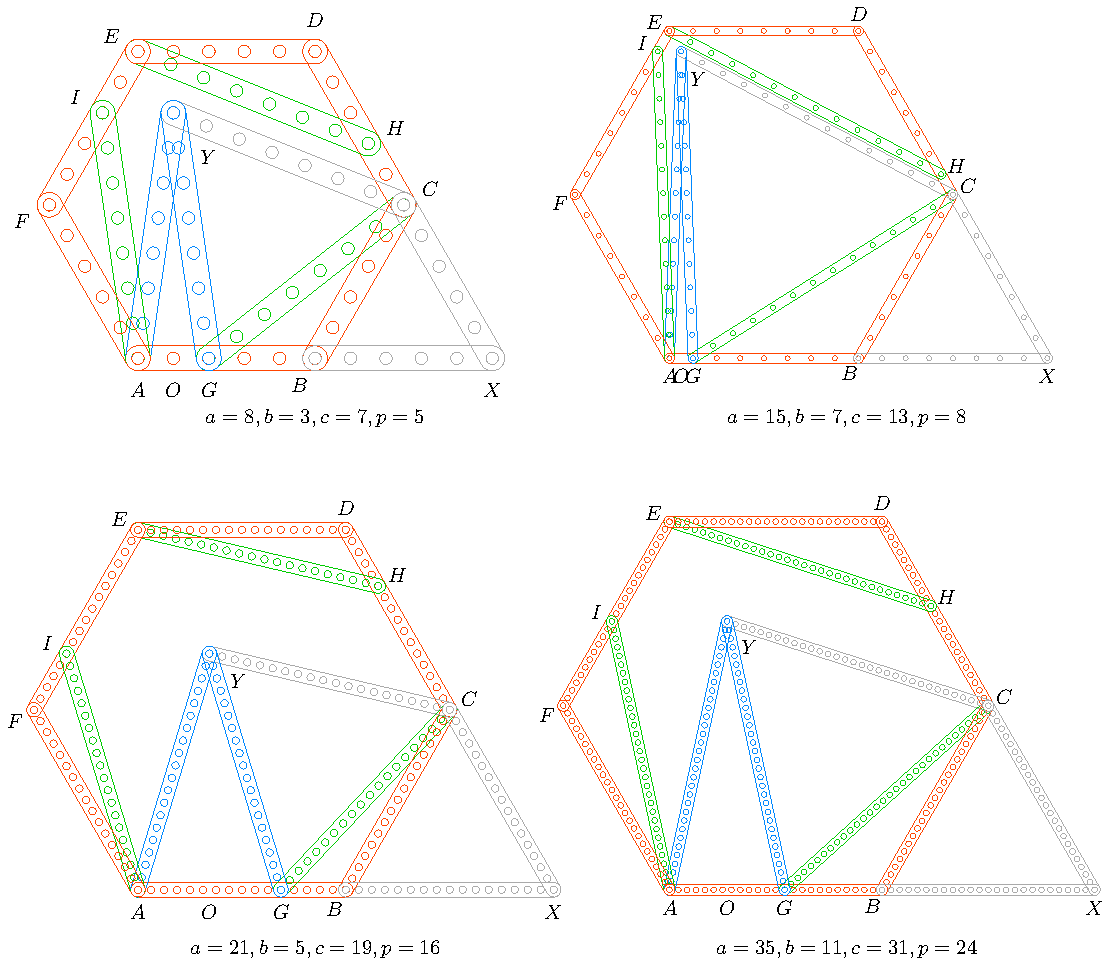
\includegraphics[scale=0.9]{build/hexa-builder-a}
\caption{First cases where internal strip $c = \overline{GC}$ is an integer and makes rigid two consecutive regular hexagon sides $s = \overline{AB} = \overline{BC}$. We use two numbers to identify every solution $a$ and $b$ where $b = \overline{GB}$ and $a = s - b$.}
\label{fig:builder-a}
\end{figure}

We run a software program to look strips that can make rigid two consecutive internal sides of any hexagon. Figure \ref{fig:builder-a} show the smaller four cases found. Consider the figure at top left, the internal hexagon angle is $\theta \equiv \angle{GBC} = 2\pi/3$ and the hexagon side is $s \equiv \overline{BC}$. Consider the triangle $\triangle{GBC}$ and define the other two sides as $b \equiv \overline{GB}$ and $c = \overline{GC}$. By the law of cosines we know that:
\begin{align}
c &= \sqrt{b^2 + s^2 - 2bs\cos\theta} \nonumber\\
 &= \sqrt{b^2 + s^2 - 2bs\left(-\frac{1}{2}\right)} \nonumber\\
 &= \sqrt{b^2 + s^2 + bs}
\end{align}
By defining $a \equiv s + b$ we get:
\begin{align}
c &= \sqrt{a^2 + b^2 - ab} \quad \texttt{ where } a > b
\end{align}
Running the software iterating first over $a$ and then by $b$ and filtering $c$ to be integer we get the first rows:
\begin{center}
\begin{tabular}{||c c c c||} 
 \hline
 $a$ & $b$ & $c$ & $s$ \\ [0.5ex] 
 \hline\hline
  8 &  3 &  7 &  5 \\ \hline
 15 &  7 & 13 &  8 \\ \hline
 21 &  5 & 19 & 16 \\ \hline
 35 & 11 & 31 & 24 \\ \hline
 40 &  7 & 37 & 33 \\ \hline
 48 & 13 & 43 & 35 \\ [1ex] 
 \hline
\end{tabular}
\end{center}


\section{Hexagons of size 13}

\end{document}
